\hypertarget{komplekse-tal}{%
\section{Komplekse Tal}\label{komplekse-tal}}

{[}{[}1 semester - erstatnings bog for - Calculus 10th
.pdf\#page=1083{]}{]}

\[w = a + ib, \s i^2 = -1\] Her er \(a\) og \(b\) \textbf{rigtige} tal.

Kan også skrives på {[}{[}\#Polær Form{]}{]}

\textbf{BRUG ALDRIG \(i = \sqrt{-1}\) SOM DEFINITION}

\[Re(w) = Re(a+ib)= a, \s Im(w) = Im(a+ib)  = b\] \textbf{Intet \(i\) i
den maginære del}

\begin{center}\rule{0.5\linewidth}{0.5pt}\end{center}

Tager udgangspunkt i {[}{[}Andengradspolynomier{]}{]} der har løsninger
hvor diskriminanten er \textbf{negativ}.

\[x = \frac{-b \pm i \sqrt{-d}}{2a}\]

\hypertarget{eksempel}{%
\subparagraph{Eksempel}\label{eksempel}}

\[2z^2 + 4z + 10 = 0\] \[d = b^2 - 4ac= -64\] Altså er dette løsningen
\[x = \frac{-b \pm i \sqrt{-(d)}}{2a} = -1 \pm 2i\]

\hypertarget{den-kompleks-konjugerede}{%
\subsubsection{Den kompleks
konjugerede}\label{den-kompleks-konjugerede}}

Hvis \(z\) er et komplekst tal af form \(z = a +ib\) den kompleks
konjugerede \(\bar{z} = a-ib\)

Hvis et polynomium med reelle koeficienter, dvs
\(x^n + bx^{n-1} + \dots\) så \(\{a,b, \dots\}\) alle er en del af
\(\R\). Har komplekse rødder, så forekommer disse altid som kompleks
konjugerede par. (F.eks. i imaginære løsninger på andengradspolynomier).

\hypertarget{muxe6ngden}{%
\subsubsection{Mængden}\label{muxe6ngden}}

\[\C\]

\hypertarget{addition}{%
\subsubsection{Addition}\label{addition}}

Hvis \(z_1 = a+ib\) og \(z_2 = c-id\), så er kan de \emph{lægges sammen}
sådan: \[z_1 + z_2 = a + ib + c-id = a+c+i(b+d)\]

\hypertarget{subtraktion}{%
\subsubsection{Subtraktion}\label{subtraktion}}

Hvis \(z_1 = a+ib\) og \(z_2 = c-id\), så er kan de \emph{trækkes fra
hinanden} sådan: \[z_1 - z_2 = a + ib - c-id = a-c+i(b-d)\]

\hypertarget{multiplikation}{%
\subsubsection{Multiplikation}\label{multiplikation}}

Hvis \(z_1 = a+ib\) og \(z_2 = c-id\), så er kan de \emph{ganges sammen}
sådan:

\[z_1 \cdot  z_2 = (a+ib)(c-id) = ac - iad + ibc + - i^2bd\]
\[ac + i^2bd + i(ac+bc)\] \(i^2 \rightarrow -1\) \[ac - bd + i(ac+bc)\]

\[z_1 \cdot  \bar{z_1} = (a+ib)(a-ib) = a^2 - i^2b^2 - \c{aib} + \c{aib} = a^2 + b^2\]
Resultater er \textbf{reelt}!

\hypertarget{division}{%
\subsubsection{Division}\label{division}}

Hvis \(z_1 = a+ib\) og \(z_2 = c+id\), så er kan de \emph{divideres}
sådan:

\[\frac{z_1}{z_2} = \frac{a + ib}{c + id}\] \textbf{Forlæger men den
kompleks konjugerede} \[\frac{(a+ib)(c-id)}{(c+id)(c-id)}\] Ganger ud
\[= \frac{ac -i^2bd + i(ab-ad)}{c^2-d^2} = \frac{ac+bd+i(bc+ad)}{c^2 + d^2}\]
Vi har no en reel (\(\R\)) nævner!

\hypertarget{poluxe6r-form}{%
\subsubsection{Polær Form}\label{poluxe6r-form}}

\hypertarget{modulus}{%
\subparagraph{Modulus}\label{modulus}}

De komplekse tal \(z=a+ib\) afbildeles i et Argand diagram . Afstanden
fra orego til punktet kaldes modulus (\(|z|\)).

\[|z| = \sqrt{a^2 + b^2}\] \#\#\#\#\# Argumentet Linjen fra orego til
punktet \((a,b)\) svarende til det komplekse tal \(z = a+ib\) danner en
vinkel med den positive del af den reelle akse (1. aksen). Vinklen
(\(\theta\)) kaldes for \emph{argumentet til \(z\)} \[arg(z) = \theta\]
(\(\theta\) skal være i intervallet \([-\pi,\pi]\))

Bestemmes således
\[arg(z)= \theta =\tan^{-1}\left(\frac{b}{a}\right) + p\pi, \s p \in \{-1,0,1\}\]

\hypertarget{poluxe6r-form-1}{%
\subparagraph{Polær form}\label{poluxe6r-form-1}}

Det komplekse tal \(z = a+ib\) med \(|z| = M\) og \(arg(z) = \theta\)
kan skrives på polær form. \[z=M\cos(\theta) + iM\sin(\theta)\] Eller
vha. eksponentialfunktion. \[z=M \cdot e^{i\theta}\]

\hypertarget{hvorfor-er-eitheta-costheta-isintheta}{%
\subparagraph{\texorpdfstring{Hvorfor er
\(e^{i\theta} = \cos(\theta) + i\sin(\theta)\)?}{Hvorfor er e\^{}\{i\textbackslash theta\} = \textbackslash cos(\textbackslash theta) + i\textbackslash sin(\textbackslash theta)?}}\label{hvorfor-er-eitheta-costheta-isintheta}}

{[}{[}Taylor Polynomier{]}{]}
\(\cos(\theta) = 1- \frac{\theta^2}{2!}-\frac{\theta^4}{4!}-\frac{\theta^6}{6!}-\frac{\theta^8}{8!}-\dots\)
\(\sin(\theta) = \frac{\theta}{1!} - \frac{\theta^3}{3!}-\frac{\theta^5}{5!}-\frac{\theta^7}{r!}-\frac{\theta^9}{9!}-\dots\)

\hypertarget{multiplikation-1}{%
\subparagraph{Multiplikation}\label{multiplikation-1}}

\[z_1 \cdot z_2 = M_1 \cdot  e^{i\theta_1} \cdot  M_2 \cdot  e^{i\theta_2} = M_1 \cdot  M_2 \cdot  e^{i(\theta_1 + \theta_2)}\]
På den anden form:
\[M_1(\cos\theta_1 + i\sin\theta_1) \cdot M_2(\cos\theta_2 + i \sin\theta_2)\]
\[\Updownarrow\]
\[M_1M_2(\cos\theta_1 \cos\theta_2 - \sin \theta_1 \sin\theta_2 + i(\sin\theta_1\cos\theta_2 + \cos\theta_1\sin\theta_2))\]
\[\Updownarrow\]
\[M_1M_2(\cos(\theta_1 + \theta_2)+i \sin(\theta_1 + \theta_2))\]
\#\#\#\#\# Division
\[\frac{z_1}{z_2} = \frac{M_1 \cdot e^{i\theta_1}}{M_2 \cdot e^{i\theta_2}} = \frac{M_1}{M_2} \cdot e^{i(\theta_1-\theta_2)}\]

\hypertarget{eksponentiering}{%
\subparagraph{Eksponentiering}\label{eksponentiering}}

\[z=M \cdot e^{i\theta}\]
\[z^n = (M \cdot e^\theta)^n = M^n \cdot e^{i\theta \cdot n} = M^n (\cos(\theta n) + i\sin(\theta n))\]

\hypertarget{de-moivres-formel}{%
\subsubsection{de Moivre's Formel}\label{de-moivres-formel}}

\[z^n = r^n \cdot (\cos(\theta) + i \cdot \sin(\theta))^n \arrow \text{Flere løsninger}\]

\[z^n = r^n \cdot (\cos(n\theta) + i \cdot \sin(n\theta)) \arrow \text{Én løsning}\]
\(r\) : længden til løsningen fra orego i det komplekse plan

\hypertarget{for-rationelle-tal}{%
\subsubsection{For rationelle tal}\label{for-rationelle-tal}}

\[z^{\frac{p}{q}} = r^{\frac{p}{q}}\cdot (\cos((\frac{p}{q} \cdot \theta) + i \sin(\frac{p}{q} \cdot \theta))\]

\hypertarget{bevis-induktion}{%
\paragraph{Bevis (induktion)}\label{bevis-induktion}}

\hypertarget{initialisering}{%
\subparagraph{Initialisering}\label{initialisering}}

\[n = 1,\s z = \cos(\theta) + i \sin(\theta)\]
\[z^1= (\cos(\theta) + i \sin(\theta))^1 \arrow \text{sandt!}\]
\#\#\#\#\# Induktions skridt \emph{Antager}: {[}{[}\#de moivre's
formel{]}{]} er sand for tallet \(k\).

Altså
\[z^k= (\cos(\theta) + i \sin(\theta))^k \arrow \text{Antages sandt}\]
Lad nu \(n = k +1\)
\[(\cos(\theta) + i \sin(\theta))^{k+1} \s=\s (\cos(\theta) + i \sin(\theta))^{k} \cdot (\cos(\theta) + i \sin(\theta))^{1}\]
Bruger de Moivre (som er antaget sandt)
\[= (\cos(k\theta) + \sin(k\theta)) \cdot (\cos(\theta) + i \sin(\theta))\]
\[= \cos(k\theta) \cdot \cos(\theta) - \sin(k\theta) \cdot \sin(\theta) + i(\cos(k\theta) \cdot \sin(\theta) + \sin(k\theta) \cdot \cos(\theta))\]
De to led kan omskrives således (blander cos og sin)
\[\cos(k\theta+\theta)+i\sin(k\theta + \theta) \s=\s \cos((k+1)\theta) + i\sin((k+1)\theta)\]
Altså (da \(n = k +1\)) \[\cos(n\theta) + i\sin(n\theta)\]

\hypertarget{komplekse-luxf8sninger}{%
\subsubsection{Komplekse løsninger}\label{komplekse-luxf8sninger}}

\begin{quote}
\emph{En ligning med kompleks løsning (eller med komplekse tal som
indgår i ligningen}
\end{quote}

Løsningers vinkel (\(\theta\)) vil altid være jævnt fordelt på den
imaginære ``cirkel''.
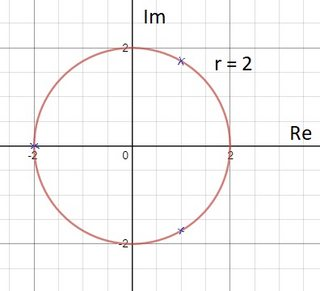
\includegraphics{https://i.stack.imgur.com/uOKmym.jpg}

\hypertarget{eksempel-1}{%
\subparagraph{Eksempel 1}\label{eksempel-1}}

Løs dette som kompleks ligning \[z^2 = 4\] 1. Bestem
{[}{[}\#Modulus{]}{]} \[|z^2| = |4| = \sqrt{4^2 + 0^2} = 4\] 2. Bestem
{[}{[}\#Argumentet{]}{]}
\[arg(z^2) = arg(4) = \tan^{-1}\left(\frac{0}{4}\right) = 0\] 3.
Opskriver løsningen på {[}{[}\#Polær form{]}{]}
\[z^2 = |z^2| (\cos(arg(z^2) + 2\pi p) + i\sin(0+2\pi p), \s p \in \Z\]
\[= 4(\cos(0 + 2\pi p) + i\sin(0+2\pi p), \s p \in \Z\] Hvis vi ser på
{[}{[}\#de Moivre's Formel{]}{]} må dette være sandt
\[z^2 \s=\s4(\cos(0 + 2\pi p) + i\sin(0+2\pi p) \s=\s r^2 (cos(2\theta) + i \sin(2\theta)), \s p \in \Z\]
Altså må dette være sandt
\[r^2 = 4 \arrow r = 2 \text{ (modulus er positivt)}, \s\]
\[2\pi p = 2\theta \arrow \pi p = \theta\] Find værdier for \(p\) der
går at \(\theta \in [-\pi, \pi]\)

\hypertarget{eksempel-2}{%
\subsubsection{Eksempel 2}\label{eksempel-2}}

\[z^3 = 27i\] 1. Beregn {[}{[}\#Modulus{]}{]}
\[|z^3| = |27i| = \sqrt{0^2+27^2} = 27\] 2. Beregn
{[}{[}\#Argumentet{]}{]} \[arg(z^3) = \frac{\pi}{2}\] Bruger {[}{[}\#de
Moivre's Formel{]}{]}
\[z^3 = 27(\cos(\frac{\pi}{2} + 2\pi p) + i\sin(\frac{\pi}{2} +2\pi p), \s p \in \Z\]
\[r^3 (cos(3\theta) + i \sin(3\theta)), \s p \in \Z \s=\s \] Sæt ind og
find værder for \(p\) og derved \(\theta\).

\hypertarget{eksempel-3}{%
\subsubsection{Eksempel 3}\label{eksempel-3}}

\[z = \cos(\theta) + i\sin(\theta)\]
\[z + \frac{1}{z} = z + z^{-1} = \cos(\theta) + {i\sin(\theta)} + \cos({-\theta}) + i\sin(-\theta) \]
Cos er lige, sin er ulige
\[\cos(\theta) + \c{i\sin(\theta)} + \cos({-\theta}) \c{- i\sin(\theta)} \]
Altså \[z + \frac{1}{z} = 2\cos{\theta}\]

\hypertarget{elektronik}{%
\subsubsection{Elektronik}\label{elektronik}}

Bruger \(j\) i elektronik.

\hypertarget{det-komplekse-plan}{%
\subsubsection{Det Komplekse Plan}\label{det-komplekse-plan}}

{[}\protect\hyperlink{det-komplekse-plan}{Det Komplekse Plan}{]}
